% !TeX spellcheck = en_GB
\chapter{Methodological Approach} \label{chap:method}

\begin{comment}
	TODO -> Update
\end{comment}

In this chapter, the problem this work aims to address is formally stated, as well as the proposed solution. In section \ref{sec:method-statement} the problem statement is exposed, section  lists the solutions main functional, non-functional and structural requirements, section \ref{sec:method-arch} addresses the architecture of the solution, section  exposes the established methodology and section  contains the proposed work plan.

\section{Problem Statement} \label{sec:method-statement}

\begin{displayquote}
	 \textit{The reviewed literature addressing solutions to sequential decision-making problems in graph-based environments is sparse and scarce, leading to a research gap for comparative and systematic \ac{GRL} approaches analysing scalability under different sized scenarios and adaptability to topology variation.}
\end{displayquote}

As addressed in the previous chapter, graphs are ubiquitous representations that can serve to instinctively represent several problems and their objects. In some network-oriented domains, these representations reveal underlying features that can't be naturally represented by plain Euclidean data. This problem becomes even more difficult considering that graph data is complex and sparse, something that brings the need for methods that efficiently extract representations. \par
By conducting a thorough literature review of the relevant studies in this context, we observed that current \ac{RL} algorithms are not as efficient as \ac{GRL} techniques in handling such complex environments, because of not considering and generalizing environment topology features in the decision-making process. This deeply affects the performance of decision systems inserted in network-oriented domains where the intricate relationships between the objects may be relevant for mapping the observable environment states to optimal action policies. \par
More and more \ac{GRL} attracts the curiosity of academics, only increasing the relevance of this problem. With the recent advancements of \acp{GNN}, the popularity around \ac{GRL} has risen because of their excellent efficiency in creating optimal graph representations and other graph machine learning problems. However, with \ac{GRL} being a field whose research is still in initial phase, the gathered literature is very sparse, with a lack of works addressing the benefits, disadvantages and performance of the various proposed models. Moreover, the literature also highlights the importance of studying \ac{GRL} models in scenarios under topology variations and of different sizes for analysing their scalability. \par

\subsection{Scope} 

This dissertation will focus on studying this problem in the context of single-agent \ac{RL} algorithms, given that multi-agent systems are significantly more complex to implement. Furthermore, in the context of the dissertation's application domain, which is smart grid services, the possible improvements in \ac{GRL} techniques will be implemented to the \acf{DED} problem that studies solutions that optimize power generation cost while maintaining reliable grid stability. Additionally, the \ac{GRL} proposed models may be also implemented to solve other smart grid systems such as Undervoltage Load Shedding and Volt-VAR Regulation. \par

\section{Problem Formalization} \label{sec:method-formal}

In this section, the main problem addressed by this dissertation is formally introduced. Firstly, it's approached from an application domain perspective concerning the \ac{DED} problem and its considered features and characteristics. In the second subsection \ref{sec:method-mdp}, the \ac{DED} problem is formalized as a dynamic sequential decision-making problem, and its characteristics are presented under the form of its corresponding \ac{MDP}. \par
These two formalizations are crucial for giving the appropriate view on how the \ac{GRL} algorithms and their environment will be approached and studied.

\subsection{Dynamic Economic Dispatch} \label{sec:method-ded}

Since the early 20th century, the improvement of power distribution grids has greatly improved society's well-being and enabled countless technological advancements. The issue of optimally distributing and accommodating customers' load demands among available power generators in an economic and reliable manner has been studied early on by academics. \cite{xiaOptimalDynamicEconomic2010}. The \acf{DED} problem addresses this concern, with a special focus on the economic factor of power systems operation. The main objective of this problem is to find the optimal dispatch strategy for the available generators that minimizes the total operating cost over a dispatch period while conforming to a particular set of constraints, such as fulfilling the total load demand of the power system. In the next subsections \ref{sec:objective-func} and \ref{sec:constraints}, the objective function and constraints considered for the \ac{DED} problem are formally introduced and further discussed.

\begin{comment}
	* Citation Needed (?)
	* Revise
\end{comment}

\begin{center}
	\begin{tabular}{ | m{2cm} | m{10cm}| } 
		\hline
		$F(t)$ & Total Operational Cost at timestep $t$ \\ 
		\hline
		$F_\text{NRES}(t)$ & Total Non-Renewable Generators Operational Cost at timestep $t$ \\
		\hline
		$F_\text{RES}(t)$ & Total Renewable Generators Operational Cost at timestep $t$  \\
		\hline
		$T$ & Terminal Timestep \\
		\hline
		$t$ & Timestep \\
		\hline
		$c^\text{NRES}_i$ & Cost of conventional generator $i$ in €/MWh \\
		\hline7
		$P^\text{NRES}_i(t)$ & Current generated power of non-renewable generator $i$ at timestep $t$ in MW \\
		\hline
		$\beta_\text{RES}$ & \ac{RES} wasted energy penalty term \\
		\hline
		$P^\text{RES}_i(t)$ & Current generated power of renewable generator $i$ at timestep $t$ in MW \\
		\hline
		$\overline{P^\text{NRES}}$, $\underline{P^\text{NRES}}$ &  Current maximum and minimum output power of non-renewable generator $i$ \\
		$\overline{P^\text{RES}_i}(t)$ &  Current maximum output power of renewable generator $i$ at timestep $t$ and before curtailment in MW \\
		\hline
		$P^\text{LOAD}_i(t)$ & Active Power demand of load $i$ at timestep $t$ \\
		\hline
		$Q^\text{LOAD}_i(t)$ & Reactive Power demand of load $i$ at timestep $t$ \\
		\hline
		$F_i$ or $F_{i,j}$ & Powerline $i$ status (connected or disconnected)\\
		\hline
		$\text{rho}_i(t)$ or $\text{rho}_{i,j}(t)$ & Relative flows of powerline $i$ or with origin in substation $i$ and destination in substation $j$. Ratio of the flow divided by its thermal limit. \\
		\hline
		$\overline{\eta_i}$, $\underline{\eta_i}$ & Maximum ramp up and down limits for non-renewable generators \\
		$P^\text{G}_i(t)$ & Current generated active power of generator $i$ in MW \\
		\hline
		$Q^\text{G}_i(t)$ & Current generated reactive power of generator $i$ in MW \\
		\hline
		$N$ & Number of non-renewable generators \\
		\hline
		$M$ & Number of renewable generators \\
		\hline
		$K$ & Number of loads \\
		\hline
		$L$ & Number of powerlines \\
		\hline
		$\theta_\text{soft}$,  $\theta_\text{hard}$ & Soft and Hard overflow thresholds \\
		\hline
		$T_\text{soft}$ & \\
		\hline
		$T_\text{reconnect}$ & \\
		\hline 
		$\overline{F_\text{NRES}}$ & \\
		\hline 
		$\overline{c^\text{NRES}}$ & \\
		\hline
	\end{tabular}
\end{center}

\subsubsection{Objective Function} \label{sec:objective-func}

As stated previously, the main goal of the \ac{DED} problem is to minimise the total cost of a power grid operation while fulfilling the total load demand over a time period $T$. The operating cost of all dispatchable generators at a timestep $t$ can be described by equation \ref{eq:conv-cost} and comprises the first component of the \ac{DED} objective function. \par

\begin{equation} \label{eq:conv-cost}
	F_\text{NRES}(t) = \sum^N_{i=0} c^\text{NRES}_i P^\text{NRES}_i(t) \Delta t
\end{equation}

In this context, conventional generation cost is described as the total sum of the generators operating cost, which in turn is described as a linear function dependent on their output value $P^\text{NRES}_i(t)$ and static cost $c^\text{NRES}_i$ in € per MWh. The reduction of the total operation cost of a power system is undoubtedly tied with the minimisation of $F_\text{NRES}(t)$, which describes a straightforward economic cost of the operation of a power grid. \par

However, more and more modern distribution grids include \acf{RES}, which also enable the manipulation of their output levels through curtailment actions. These acts allow the power system to adapt to its dynamic needs associated with reliability, stability, and security by adjusting the maximum output of \ac{RES}. Regardless of its contributions, curtailment does not come without its disadvantages, mainly connected with the hidden cost of curtailed (unused) \ac{RES} energy that might be transferred to other generators' operations for security reasons, such as preventing line overflow. \par

In this manner, as a means of maximising the \ac{RES} usage, a second component of the objective function is considered that focuses on expressing this cost, represented in equation \ref{eq:res-cost}. A penalty factor $\beta_\text{RES}$ controls the influence of wasted \ac{RES} energy on the overall objective. Additionally, this work considered another element representing the average cost $\overline{c^\text{NRES}_i}$ of conventional generators as the cost of the abandoned \ac{RES} energy. This creates a more understandable and comparable definition of the total operating cost of renewable generators.  \par

\begin{equation} \label{eq:res-cost}
	F_\text{RES}(t) = \beta_\text{RES} \sum^M_{i=0}  (\overline{P^\text{RES}_i}(t) - P^\text{RES}_i(t)) \Delta t 
\end{equation}

Finally, the primary objective function of \ac{DED} can be defined by minimising the total sum of both components $F_\text{NRES}(t)$ and $F_\text{RES}(t)$ for the period $T$. This is clearly stated in equation \ref{eq:ded-function}.

\begin{equation} \label{eq:ded-function}
	\min F (t) =  \min\sum^T_{t=1}(F_\text{NRES}(t) + F_{\text{RES}}(t)
\end{equation}

\subsubsection{Constraints} \label{sec:constraints}

In order to maintain stability and reliable power distribution, the system must follow several operational constraints. These restrictions are related to generators, voltage, powerlines and overall stability.  \par

The primary constraint considered in \ac{DED} consists of compliance with power balance. This implies that, at all times, the sum of the production output of all generators must surpass the total system load demand, as portrayed by equation \ref{eq:c-power-balance} \cite{}. 

\begin{equation} \label{eq:c-power-balance}
	\sum^N_i P^\text{NRES}_i(t) + \sum^M_i P^\text{RES}_i(t) = \sum^L_i P^\text{LOAD}_i(t) + \delta, \delta > 0
\end{equation}

Another equally important group of constraints is the Kirchoff's Laws of current and voltage. These fundamental principles establish the foundational rules that govern the behaviour of electrical circuits and power networks. The Kirchoff's voltage law, represented by equation \ref{eq:kirchoff-volt}, determines that the sum of all electrical potentials around a closed circuit loop must equal zero, ensuring that all voltages are consistent and feasible. On the other hand, the Kirchoff's current law, illustrated in equation \ref{eq:kirchoff-curr}, dictates that the sum of all currents entering and leaving any node in a power networks must equal zero to guarantee that the conservation of energy is respected. 

\begin{equation} \label{eq:kirchoff-volt}
	\sum_{k=1}^n  V_k = 0
\end{equation}

\begin{equation} \label{eq:kirchoff-curr}
	\sum_{k=1}^n  I_k = 0
\end{equation}


Regarding non-renewable generators, their output value is bounded by absolute maximum and minimum values respective to each generator, $\underline{P^\text{NRES}_i}$ and $\overline{P^\text{NRES}_i}$, as depicted in equation \ref{eq:prod-limits}. Furthermore, as illustrated by equation \ref{eq:ramp-limits}, the varying power between two different timesteps is also restricted by the maximum ramp-up and down limits, $\underline{\eta_i }$ and $\overline{\eta_i }$. \par

\begin{equation} \label{eq:prod-limits}
	\forall t, i: \underline{P^\text{NRES}_i} \leq P^\text{NRES}_i(t) \leq \overline{P^\text{NRES}_i}
\end{equation}

\begin{equation} \label{eq:ramp-limits}
	\forall t, i: \underline{\eta_i } \Delta t \leq P^\text{NRES}_i (t + 1) - P^\text{NRES}_i (t) \leq \overline{\eta_i} \Delta t
\end{equation}

In contrast with these static production limits, renewable generator production has a dynamic maximum output level and is not bounded by ramp rate limits. Depending on the type of \ac{RES}, its maximum generation output is inherently tied to the environmental conditions that support its operation. These conditions, such as the availability of natural inputs, climate and other local dynamic factors, determine the efficiency and capacity at which the renewable sources operate. In such manner and as equation \ref{eq:res-limits} portrays, the output value of renewable generations for any timestep $t$ is bounded by a maximum production value, $\overline{P^\text{RES}_i} (t)$ and 0.

\begin{equation} \label{eq:res-limits}
	\forall t, i: 0 \leq P^\text{RES}_i (t) \leq \overline{P^\text{RES}_i} (t)
\end{equation}

Regarding powerlines, there is several restrictions in their dynamic operation that aim to consider the real behaviour of power systems. There are two main thresholds associated with two real-world scenarios:

\begin{itemize}
	\item \textbf{Hard Overflow} - In case the relative flow of any powerline surpasses the hard overflow threshold, $\theta_\text{hard},$ it's instantly disconnected. This corresponds to a instantenous overcurrent and prevents the power system from operating in cases of extreme overflow;
	\item \textbf{Soft Overflow} - A line is allowed to surpass the soft overflow threshold, $\theta_\text{soft}$, for $T_\text{soft}$ timesteps before being disconnected for safety reasons. This consists in an time overcurrent and describes the level at which a line is allowed to be in overflow for maximum amount of time;
\end{itemize}
Regardless of the scenario, when a powerline is disconnected for safety reasons, it's always affected by a reconnection cooldown, $T_\text{reconnect}$.

\begin{comment}
	Voltage Constraints ? 
\end{comment}

\subsection{\acf{MDP}} \label{sec:method-mdp}

In this section, the \ac{DED} problem is formalized as a sequential decision-making problem and its \ac{MDP} is uncovered. This is necessary to approach \ac{DED} as a \ac{RL} problem and propose an appropriate solution. 

\begin{description}
	\item[Action] The considered action space includes the change in conventional generator redispatching $\Delta P^\text{NRES}_i$ and the renewable energy curtailment $P^\text{RES}_i$. The first concerns only non-renewable dispatchable generators and is done in increments and decrements. At the same time, the second is the ratio of curtailment applied to the total amount of generation output of a renewable generator. \par
	This second type of action refers to the energy discarded from \ac{RES} for grid stability and security purposes. However, they're represented as the upper bound on a renewable generator's output level. In this manner, while positive dispatch actions are directly tied with higher energy output and, consequently, the operational cost of the system, curtailment actions have the opposite effect, given that they are represented as the upper bound on renewable generator output levels. Therefore, higher curtailment values reduce the wasted energy provided from \ac{RES}, making these actions crucial for an optimal grid operation.
	
	\begin{equation} \label{eq:action-space}
		A = \{P^\text{NRES}_1, P^\text{NRES}_2, \dots, P^\text{NRES}_N, P^\text{RES}_1, P^\text{RES}_2, \dots, P^\text{RES}_M\}
	\end{equation}
	
	\item[Observation] The observation space is composed of four components concerning Generators, \ac{RES}, Loads and Powerlines. The relevant characteristics were included in the action space highlighted by the following equations:
	
	\begin{equation} \label{eq:simple-obs-space1}
		o_{1}(t)= \begin{bmatrix}
			P^\text{NRES}_1 & P^\text{NRES}_2 & \dots & P^\text{NRES}_{N} \\
		\end{bmatrix}
	\end{equation}
	
	\begin{equation} \label{eq:simple-obs-space2}
		o_{2}(t)= \begin{bmatrix}
			P^\text{RES}_1 & P^\text{RES}_2 & \dots & P^\text{RES}_{M} \\
			\overline{P^\text{RES}_1} & \overline{P^\text{RES}_2} & \dots & \overline{P^\text{RES}_{M}} \\
		\end{bmatrix}
	\end{equation}
	
	\begin{equation} \label{eq:simple-obs-space3}
		o_{3}(t)= \begin{bmatrix}
			P^\text{LOAD}_1 & P^\text{LOAD}_2 & \dots & P^\text{LOAD}_{K} \\
			Q^\text{LOAD}_1 & Q^\text{LOAD}_2 & \dots & Q^\text{LOAD}_{K} \\
		\end{bmatrix}
	\end{equation}
	
	\begin{equation} \label{eq:simple-obs-space4}
		o_{4}(t)= \begin{bmatrix}
			F_1 & F_2 & \dots & F_{L} \\
			\text{rho}_1 & \text{rho}_2 & \dots & \text{rho}_{L} \\
		\end{bmatrix}
	\end{equation}
	
	\begin{equation} \label{eq:simple-obs-space}
		o(t)= \{ o_{1}(t), o_{2}(t), o_{3}(t), o_{4}(t) \}
	\end{equation}
	
	This tuple encompasses the main elements of the power grid and their characteristics without capturing their topology. This is the space considered for pure-\ac{DRL} baselines, and it was taken from similar literature that addresses \ac{DED} with equivalent considerations. \par 
	Concerning the network's topology, for \ac{GRL} algorithms, this tuple was replaced by a graph structure representing the power grid configuration. This graph is defined by its adjacency, weight, and feature matrix and its feature tuple for node $i$ at timestep $t$ can be observed in equation \ref{eq:graph-obs-space}. 
	
	\begin{equation} \label{eq:graph-obs-space}
		o_i(t) = \{P^\text{LOAD}_i, Q^\text{LOAD}_i, P^\text{NRES}_i, P^\text{RES}_i, \overline{P^\text{RES}_i}, t\}
	\end{equation}
	
	In this context, the features are aggregated along the existent nodes which may have several connected elements such as loads and generators. The adjacency matrix is derived from \textit{line status} and the weight matrix corresponds to th \textit{rho} value of each line. Finally, a graph representation is obtained from the initial equation \ref{eq:simple-obs-space}, enabling their exploit and posterior study by \ac{GRL} algorithms.
	
	\begin{equation}
		o(t) = G(\text{Adj}, W, X)
	\end{equation}
	
	where,
	
	\begin{equation}
		\text{Adj}_{i,j} = F_{i,j}
	\end{equation}
	
	\begin{equation}
		W_{i,j} = \text{rho}_{i,j}
	\end{equation}
	
	\begin{equation}
		X_i = o_i
	\end{equation}
	
	\begin{comment}
		* REFERENCE
		* GNN Equations
	\end{comment}
	
	\item[Reward] Considering reward functions, three formalizations were considered. The initial implementation can be described by equation \ref{eq:reward1} and corresponds to the total amount of cost saved at time step $t$, with the maximum cost, $\overline{F_\text{NRES}}$, representing the total cost of running the power system for the current step with all generators running at maximum output. \par
	
	
	\begin{equation} \label{eq:reward1}
		\begin{split}
			r_1(t) &= \overline{F_\text{NRES}} - F_\text{NRES}(t) \\
			&= \overline{F_\text{NRES}} - \sum^N_{i=0} c^\text{NRES}_i P^\text{NRES}_i(t) \Delta t
		\end{split}
	\end{equation}
	
	This definition aims to encompass the main objective of \ac{DED}, directly tying reward maximization and the reduction of operation cost. In this manner, the reward represents an estimate of the system expense over a timestep in €. However, it disregards a secondary objective concerning the maximization of \ac{RES} generated energy. \par
	In this context, another component is added to consider the cost of wasted \ac{RES} energy, depicted in equation \ref{eq:reward2-pen}. This cost is calculated using the average cost per MW of all non-renewable generators of the system, $\overline{c^\text{NRES}}$, and a penalty factor, $\beta_\text{RES}$, to control the impact of wasted energy in reward value. \par
	
	\begin{equation} \label{eq:reward2-pen}
		\begin{split}
			r_2(t) &= - F_\text{RES}(t) \\
			&= \overline{c^\text{NRES}} \beta_\text{RES} \sum^M_{i=0} (\overline{P^\text{RES}_i}(t) - P^\text{RES}_i(t)) \Delta t 
		\end{split}
	\end{equation}
	
	In addition, this component was also idealized as a bonus instead of a penalty. In contrast with the last definition, the maximization of renewable energy can also be considered through a positive reward for its utilization instead of penalizing its waste. This second version of the \ac{RES} component can be observed in equation \ref{eq:reward2-bon}\par
	
	\begin{equation} \label{eq:reward2-bon}
		r_2(t) = \overline{c^\text{NRES}} \beta_\text{RES} \sum^M_{i=0} P^\text{RES}_i(t) \Delta t 
	\end{equation}
	
	\begin{equation}
		r(t) = r_1(t) + r_2(t)
	\end{equation}
	
	\item[Invalid Actions and Game Over] In the context of the power system simulation, there are some considerations accounting to invalid actions and errors that cause a terminal state of the system or a \textit{game over}. If at any timestep the power system reaches an infeasible state there is a game over and the episode ends. These happen any time there's no following action that conforms to the contraints of power balance and the Kirchoff's laws. In this case, the reward at the timestep it happens is minimum (-1). \par
	At any other case when actions don't respect the other considered constraints related to the power output, ramp limits and powerlines, the action is considered invalid and the returned reward is zero.
	
	
	\item[Episodes and Steps] Considering the time difference between the two steps, each timestep represents a five-minute period where the environmental characteristics remain constant. Furthermore, the length of an episode corresponds to a week of operation, which in turn translates into 2016 timesteps. \par

	
	\begin{equation}
		\Delta t = 300 s
	\end{equation}
	
	\begin{equation}
		\text{Episodic Length} = 2016 t
	\end{equation}
	
\end{description}

\section{Device Specifications} \label{sec:method-specs}

The experiments were executed on two different machines, the author's own and a remote server made available by LIACC (\textit{Laboratório de Inteligência Artificial e Ciência de Computadores}). Tables \ref{tab:specs-msi} and \ref{tab:specs-liacc} highlight their hardware specifications.

\begin{table} 
	\begin{tabular}{|l|l|}
		\hline
		OS & Arch Linux \\
		Kernel & 6.10.6-zen1-1-zen \\
		CPU & Intel i7-9750 @ 4.5 GHz \\
		GPU & Nvidia GeForce GTX 1650 Mobile / Max-Q \\
		GPU Memory & 4 GB  \\
		Driver Version & 555.58.02 \\
		CUDA Version & 12.5 \\
		RAM & 16 GB \\
		\hline
	\end{tabular}
\caption{MSI Laptop Specifications}
\label{tab:specs-msi}
\end{table}

\begin{table} 
	\begin{tabular}{|l|l|}
		\hline
		OS & Ubuntu 20.04.1 \\
		Kernel & 5.15.0-117-generic \\
		CPU & 13th Gen Intel(R) Core i7-13700K @ 5.4 GHz \\
		GPU & NVIDIA RTX A6000 \\
		GPU Memory & 48 GB \\
		Driver Version & 535.183.01 \\
		CUDA Version & 12.2 \\
		RAM & 62 GB \\
		\hline
\end{tabular}
\caption{LIACC Server Specifications}
\label{tab:specs-liacc}
\end{table}

\section{Technologies} \label{sec:method-technologies}

Beyond being a well-documented, fast, robust and modular language, \textit{Python} is an ubiquitous technology for implementing machine learning algorithms. Furthermore, the main libraries used to implement the simulation environment and algorithm are native to this language. \par
In table x, the main requirements for the project can be observed, along with their respective version number and a short description of their purpose and functionality.
\par

\begin{table}
	\begin{tabular}{|l|l|l|}
		\hline
		\textbf{Name} & \textbf{Description} & \textbf{Version Number} \\
		\hline
		Python & Functional Programming Language & 3.11.9 \\
		\hline
		Numpy & Numerical Computing Library& 1.24.3 \\
		\hline
		Ray & Used for hyperparameter tuning & 2.21.0 \\
		\hline
		PyTorch & \acs{ML} Library used by stable-baselines3 & 2.3.0 \\
		\hline
		PyTorch Geometric & \ac{GNN} Implementations & 2.5.3 \\
		\hline
		Grid2Op & Power Grid Simulation Platform & 1.9.8 \\
		\hline
		Pandas & Data Manipulation and Analysis & 1.5.3 \\
		\hline
		LightSim2Grid & Fast Grid2Op Backend & 0.8.2 \\
		\hline
		Gymnasium & \ac{RL} Single-Agent API & 0.29.1 \\
		\hline
		Stable Baselines 3 & \ac{DRL} Implementations & 2.3.2 \\
		\hline
	\end{tabular}
	\caption{Project Requirements}
\end{table}

Grid2Op is a critical requirement used to simulate the power grid operation in different manageable scenarios. This is further discussed in the next subsection \ref{sec:method-environment}. Stable-Baselines3 was chosen for its performance, customization and descriptive documentation, while PyTorch Geometric was favoured because of the wide variety of \acp{GNN} Implementations included. Additionally, these libraries mix well because stable-baselines3 already uses PyTorch in its \ac{DRL} implementations.
\par
Lastly, \textit{Gymnasium} is used as the standard \ac{RL} single-agent API in the entirety of the project, adding robustness, scalability and flexibility to agent-environment interaction process in the implementation.  \par

\section{Simulation Environment} \label{sec:method-environment}

The \textit{Grid2Op} framework \cite{rtefranceGrid2OpDocumentation} will be used for modelling the sequential decision-making process on simulated power distribution grids. \textit{Grid2Op} is designed by RTE (\textit{Réseau de Transport d'Électricité}), the electricity transmission system operator of France, and is equipped with a variety of pre-defined scenarios used in coding competitions and based on real-world data \cite{rtefranceGrid2OpDocumentation}. \par
This \textit{python} library implements the creation of power grid environments that emulate a subset of the elements and physical constraints of real power systems. On one hand, the main objects and their interactions are captured realistically, while on the other, the abstraction level used to model the fundamental elements of a power grid facilitates the implementation of intelligent systems in safe and controllable scenarios. \par
Furthermore, \textit{Grid2Op} models the dynamic topology of power systems as graph-structured data, which also eases the study of how this information can influence decision-making systems performing on these environments.  In figure \ref{fig:grid2op-graph}, a graphical plot of the environment state at an arbitrary timestep can be observed. \par
This framework is compatible with the \textit{Gymnasium} framework \cite{faramafoundationGymnasiumDocumentation}, a widely used toolkit for developing \ac{RL} algorithms, which will also will be used in this work together with the Grid2Op simulation environment. 

\begin{itemize}
	\item redispatch - change the production output of non-renewable generators in incrementing or decrementing intervals 
	\item curtail - change the production setpoint of renewable generators bellow the current maximum available power \cite{rtefranceGrid2OpDocumentation}
\end{itemize}



\begin{figure}
	\centering
	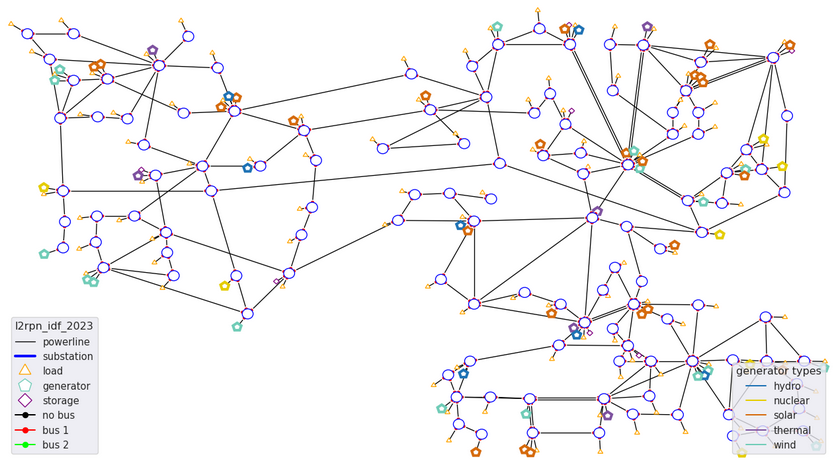
\includegraphics[width=0.85\linewidth]{./figures/grid2op-graph.png}
	\caption{Grid2Op \textit{l2rpn\_idf\_2023} 118-bus test case \cite{rtefranceGrid2OpDocumentation}}
	\label{fig:grid2op-graph}
\end{figure}


\subsection{Elements}

The main elements that are modelled by the simulation environment are presented in this subsection. The power grid is reduced to its fundamental components and their properties:

\begin{itemize}
	\item \textbf{Buses} are the fundamental objects of the power grid, representing nodes where power sources, loads and other elements are connected\cite{rtefranceGrid2OpDocumentation}.
	
	\item \textbf{Powerlines} represent edges in the power grid and connect the different buses together. They represent the physical transmission and distribution lines and allow power to flow from one part of the grid to another \cite{rtefranceGrid2OpDocumentation}.
	\begin{itemize}
		\item status
		\item rho
	\end{itemize}
	
	\item \textbf{Generators} are critical grid elements connected to buses whose main role is to produce power and maintain grid stability by balancing the energy supply and demand. They can be Conventional Thermal Generators, Wind Turbines or Photovoltaic Cells \cite{rtefranceGrid2OpDocumentation}.
	\begin{itemize}
		\item $P^\text{NRES}_i(t)$ - Power generation at non-renewable generator $i$
		\item $P^\text{RES}_i(t)$ - Power generation at renewable generator $i$
		\item $\overline{P^\text{RES}_i}(t)$ - Maximum power generation at renewable generator $i$
		\item $\overline{P^\text{NRES}_i}, \underline{P^\text{NRES}_i}$ - Maximum/Minimum power generation at renewable generator $i$
	\end{itemize}
	
	
	\item \textbf{Loads} consume power from the grid, simulating electricity use. They're also associated to an individual bus \cite{rtefranceGrid2OpDocumentation}.
	\begin{itemize}
		\item $P^\text{LOAD}_i$ - Active power at load $i$
		\item $Q^\text{LOAD}_i$ - Reactive power at load $i$
	\end{itemize}
	
	\item \textbf{Storage Units} can act as both consumers and producers. They're able to retain energy from the power grid when production surpasses demand for later injecting back power when convenient. Storage units are bound by a maximum energy storage capacity \cite{rtefranceGrid2OpDocumentation}.
\end{itemize}


Beyond \textit{grid2op} to build and run the test cases and \textit{gymnasium} as the RL framework, this project will use \textit{PyTorch} \cite{pytorchPyTorch} with \textit{PyTorch Geometric} \cite{pygteamPyGPytorch_geometric} library for developing the \ac{GNN} because of its extensive list of available implemented models. The different combinations of algorithms will be applied to a set of modified scenarios that fulfil the settled requirements. For Deep Reinforcement Learning algorithms, solutions with plain \ac{SAC}, \ac{DDPG} and \ac{PPO} approaches and combined with the \ac{GCN}, \ac{GAT} and \ac{GIN} architectures.  \par
Concerning result analysis, it's also important to point out the use of quantitative methods for evaluating the different implemented models, a topic that is further explored in the following section \ref{sec:method-eval}.

\subsection{Parameters}

Grid2Op also defines a number of customizable environment parameters that control some very important grid properties and settle some bounds on the agent-envrionment interaction. As there is a significant number of parameters that consider details that are out of the scope of this project, only the relevant parameters are exposed in table \ref{tab:grid-params}.

\begin{table}[H] 
	\centering
	\caption{Grid2Op Relevant Parameters}
	\begin{tabular}{|p{6.5cm}|p{6cm} | p{2cm} |}
		\hline
		\textbf{Parameter} & \textbf{Description} & \textbf{Default} \\
		\hline
		\texttt{NO\_OVERFLOW\_DISCONNECTION} & If \texttt{true}, the powerlines over their thermal limit will never be disconnected & \texttt{false} \\
		\hline
		\texttt{NB\_TIMESTEP\_OVERFLOW\_ALLOWED} & Number of timesteps a powerline is allowed to be in a soft overflow before it gets disconnected by time overcurrent & 2 \\
		\hline
		\texttt{NB\_TIMESTEP\_RECONNECTION} & Number of timesteps that a line disconnected for security reasons will stay disconnected & 10 \\
		\hline
		\texttt{HARD\_OVERFLOW\_THRESHOLD} & If the power flow of a line is above the settled hard overflow threshold it's instantaneously and automatically disconnected & 2.0 \\
		\hline
		\texttt{SOFT\_OVERFLOW\_THRESHOLD} & If the power flow of a line is above the defined soft overflow threshold for over \texttt{NB\_TIMESTEP\_OVERFLOW\_ALLOWED} steps, it's automatically disconnected & 1.0 \\
		\hline
		\texttt{ENV\_DC} & If \texttt{true}, the environment will use direct current approximations instead of alternative current & \texttt{false} \\
		\hline
		\texttt{LIMIT\_INFEASIBLE\_CURTAILMENT\_ STORAGE\_ACTION} & If set to \texttt{true}, the environment will automatically limit curtailment (and storage) actions that otherwise would lead to an infeasible system state. Might help the training and learning process of the model and significantly increases the survivability of the agent & \texttt{false} \\
		\hline
	\end{tabular}
	\label{tab:grid-params}
\end{table}

Most of the parameters, with the exception of one, were left at their default values depicted in table \ref{tab:grid-params}. This includes the overflow thresholds, all of the timestep limits mentioned and direct current flag, whose values were found to be sensible enough to maintain a realistic yet feasible model of the environment. The only parameter that was tampered was \texttt{LIMIT\_INFEASIBLE\_CURTAILMENT\_STORAGE\_ACTION} with the goal of improving the learning efficency of the algorithms during training.

\subsection{Scenarios} 

\begin{table}[H] 
	\centering
	\caption{Test Case Sizes}
	\begin{tabular}{|P{2cm}|P{3.5cm}|P{4cm}|P{3.5cm}| }
		\hline
		& \textbf{l2rpn\_case14\_sanbox} & \textbf{l2rpn\_icaps\_2021\_large} & \textbf{l2rpn\_idf\_2023} \\
		\hline
		\textbf{Buses} & 14 & 36 & 118 \\
		\hline
		\textbf{Powerlines} & 20 & 59  & 186  \\
		\hline
		\textbf{Generators} & 6 & 22 & 62  \\
		\hline
		\textbf{Loads} & 11 & 37 & 99 \\
		\hline
		\textbf{Episodes} & 1004 & 2952 & 832 \\
		\hline 
	\end{tabular}
	\label{tab:test-case}
\end{table}

This work will use the pre-defined \textit{grid2op} \textit{l2rpn\_case14\_sandbox}, \textit{l2rpn\_icaps\_2021\_large} and \textit{l2rpn\_idf\_2023} test environments. The scenarios define the properties and characteristics of loads and generators at each time step, as well as the grid layout \cite{rtefranceGrid2OpDocumentation} for weekly episodes. The data from the scenarios is non-continuous, with each episode being independent of the others in its original sequence (and they are also shuffled in practice). The test cases' characteristics can be further observed in table \ref{tab:test-case}. \par
The first case was used for the primary implementation and development of the algorithms, given its small grid size. Motivated by its considerable grid size and amount of training data, the second test case was mainly used for the calibration of the model's main parameters. It's a subset of the original 118-bus system \cite{christiePowerSystemsTesta} with 50 years' worth of data divided into independent \footnote{non-consecutive} weekly scenarios. Finally, the third scenario is based on the same original test case as the previous one, and it includes modifications that aim to accommodate the \textit{possible energy mix} of France in 2035, containing 16 years of data \cite{rtefranceGrid2OpDocumentation}. It was mainly used to study the algorithm's scalability and performance in larger scenarios in comparison with the baseline plain-\ac{DRL} model. \par


\section{Solution Architecture} \label{sec:method-arch}

Considering the conclusions taken from the reviewed literature, in chapter \ref{chap:review}, our proposed solution combines efficient \acf{DRL} approaches with \acfp{GNN}, the state-of-the-art approach for graph representation learning. Generally, the system receives graph-based representations of the environment and encodes them using the \ac{GNN} algorithm. By also leveraging deep learning techniques, \ac{DRL} maps the encoded embeddings to optimal action sequences with the goal of meeting the real-time load demand and reducing the operating cost of the power distribution grid. The general architecture of the solution can be observed in figure \ref{fig:arch}.

\begin{figure}
	\centering
	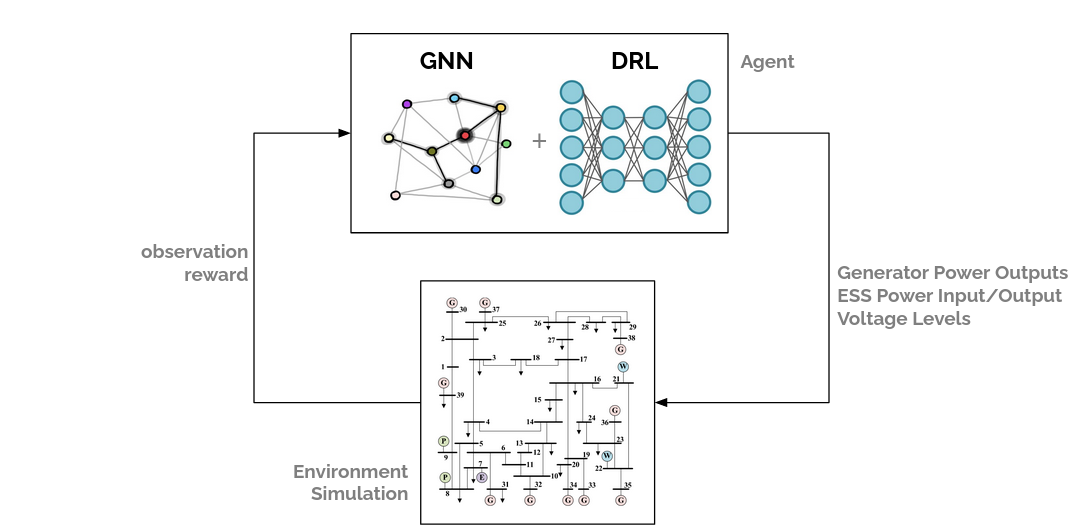
\includegraphics[width=0.85\linewidth]{./figures/arch.png}
	\caption{Solution Architecture}
	\label{fig:arch}
\end{figure}


To fulfil this, the agent adjusts the generator power output and voltage levels and manages the \ac{ESS} operation in real-time. The proposed solution is trained and tested in a power grid simulation that models the appropriate elements, properties, constraints and operation of the power distribution grid. \par
In order to achieve this purpose, the \ac{GRL} models were implemented using \textit{stable-baselines3} \ac{DRL} implementations and \textit{torch\_geometric} \ac{GNN} models. Beyond having several different implementations available for both their respective types of algorithms, utilizing these two technologies simplifies the integration of models from each, allowing for more straightforward testing of various combinations. \par
Although stable-baselines3 allows for the implementation of custom feature extractors, this method was not computationally optimal. \ac{DRL} models of this library that use mini-batching have an increased complexity due to the extractor being called on each batch observation at every step. This issue is derived from another problem which is obviously the storage of raw observations in the replay buffer, where the data is batched from, instead of the extracted features.To solve this, the \ac{GNN} feature extraction layer was included directly in the observation space which ensured the execution of module only once per step. \par



\section{Evaluation Metrics} \label{sec:method-eval}


The solution described in the previous subsection \ref{sec:method-arch} involves intricate operational mechanisms, something that calls for a sophisticated evaluative and test process. Furthermore, given this dissertation's comparative nature, the evaluation and analysis methods will be critical factors in studying and confronting the different combinations of \acp{GNN} and \ac{DRL}, as well as possible improvements in integrating these techniques. In this manner, we define the six dimensions for evaluating and analysing the different \ac{GRL} models:

\begin{description}
	\item[Learning efficiency] This dimension assesses how effectively the models learn and improve their decision-making process over time. It involves evaluating how quickly they converge to optimal or near-optimal dispatch strategies through the convergence rate. This is mainly assessed by analysing the evolution of episodic accumulative reward over the training process.
	
	\item[Dispatch Efficiency] The performance of the \ac{GRL} model in managing power distribution from the various generators will be mainly measured by the average operating cost (in \textit{Euros}) derived from the agent's sequence. 
	
	\item[Abandoned RES] An important factor to take into consideration is the wasted \ac{RES} energy. The models will be analysed on their \ac{RES} penetration the average unused \ac{RES} power.
	
	\item[Survivability] Although the primary objective of \ac{DED} focuses on the economic performance of a power system, a model must successfully meet the specified constraints and complete episodes in order to accurately determine optimal dispatch strategies and understand the correlations with environmental dynamics. \par
	In this context, the survivability of models must be addressed and improved in order to maintain grid reliability, stability, and security beyond an economic operation. \par
	This factor is evaluated through the survival rate metric, which represents the percentage of maximum episode length the model is able to survive.
	
	\item[Scalability]  The solution will be tested on scenarios of various sizes to analyse its scalability. This is a crucial factor for comparing the \ac{GRL} and pure-\ac{DRL} approaches, as the literature suggests that the former is more scalable and adaptable to changes in topology.
	
	\item[Computational Efficiency] It is crucial that the solution is able to perform well in real-time execution. In this context, it's important to assess the solution's decision computation performance and measure the time necessary for the model offline training and the observed CPU/GPU resource utilisation.
\end{description}
	
	To ensure an unbiased evaluation of the proposed models, the data from the scenarios is divided into training and testing samples with a 90-10 ratio. Given the complexity of the problem and the limited data available, this split allows for a sufficient number of episodes to effectively learn optimal policies during training while still providing a representative and robust, albeit small, test sample to evaluate the model's performance and generalisation capability. Additionally, cross-validation was considered, but its use was discarded because of the algorithms' slow performance and apparent reduced learning efficiency.
